% ============================================================
%  Présentation du cours — Développement Web — Classe passerelle
%  PRÉSENTATION D'OUVERTURE (Beamer) — cfpt·i | Anne Terrier
%  Version courte : 10 diapositives, ~15 minutes.
%  À projeter en ouverture de la première séance,
%  avant S01_presentation.tex (contenu technique de la semaine 1).
% ============================================================
\documentclass[aspectratio=169,11pt]{beamer}

\usepackage[T1]{fontenc}
\usepackage[utf8]{inputenc}
\usepackage[scaled=0.92]{helvet}
\renewcommand{\familydefault}{\sfdefault}

\usepackage{tikz}
\usetikzlibrary{positioning, arrows.meta}
\usepackage{booktabs}
\usepackage{tabularx}
\usepackage{colortbl}

% ---------------------------------------------------------------
% Palette cfpt·i
% ---------------------------------------------------------------
\definecolor{cfptYellow}{HTML}{F5C400}
\definecolor{cfptBlack}{HTML}{1A1A1A}
\definecolor{cfptDarkGrey}{HTML}{555555}
\definecolor{cfptGrey}{HTML}{F2F2F2}
\definecolor{accentBlue}{HTML}{1D4E89}
\definecolor{lightBlue}{HTML}{D6E4F0}
\definecolor{successGreen}{HTML}{1E7145}
\definecolor{warningOrange}{HTML}{C55A11}
\definecolor{alertRed}{HTML}{A32020}

% ---------------------------------------------------------------
% Thème Beamer personnalisé cfpt·i
% ---------------------------------------------------------------
\usetheme{default}
\usecolortheme{default}
\setbeamercolor{palette primary}{bg=accentBlue, fg=white}
\setbeamercolor{structure}{fg=accentBlue}
\setbeamercolor{frametitle}{bg=accentBlue, fg=white}
\setbeamercolor{title}{fg=white}
\setbeamercolor{block title}{bg=accentBlue, fg=white}
\setbeamercolor{block body}{bg=lightBlue!30, fg=cfptBlack}
\setbeamercolor{block title alerted}{bg=cfptYellow!85!black, fg=cfptBlack}
\setbeamercolor{block body alerted}{bg=cfptYellow!20, fg=cfptBlack}
\setbeamercolor{block title example}{bg=successGreen, fg=white}
\setbeamercolor{block body example}{bg=successGreen!8, fg=cfptBlack}
\setbeamercolor{itemize item}{fg=cfptYellow!85!black}
\setbeamercolor{itemize subitem}{fg=cfptDarkGrey}
\setbeamercolor{normal text}{fg=cfptBlack}
\setbeamercolor{footline}{fg=white}

\setbeamertemplate{itemize item}{\textbullet}
\setbeamertemplate{itemize subitem}{--}
\setbeamertemplate{navigation symbols}{}
\setbeamertemplate{blocks}[rounded][shadow=false]

% Titre de frame : bandeau plein largeur
\setbeamertemplate{frametitle}{%
  \nointerlineskip%
  \begin{beamercolorbox}[wd=\paperwidth, ht=2.6ex, dp=1.2ex, leftskip=0.3cm]{frametitle}%
    \usebeamerfont{frametitle}\bfseries\insertframetitle%
  \end{beamercolorbox}%
}

% Pied de page
\setbeamertemplate{footline}{%
  \leavevmode%
  \hbox{%
    \begin{beamercolorbox}[wd=.32\paperwidth, ht=2.4ex, dp=1ex, leftskip=0.3cm]{palette primary}%
      \usebeamerfont{author in head/foot}\tiny Anne Terrier%
    \end{beamercolorbox}%
    \begin{beamercolorbox}[wd=.44\paperwidth, ht=2.4ex, dp=1ex, center]{palette primary}%
      \usebeamerfont{title in head/foot}\tiny Développement Web --- Classe passerelle%
    \end{beamercolorbox}%
    \begin{beamercolorbox}[wd=.24\paperwidth, ht=2.4ex, dp=1ex, right, rightskip=0.3cm]{palette primary}%
      \usebeamerfont{date in head/foot}\tiny\insertframenumber\,/\,\inserttotalframenumber%
    \end{beamercolorbox}%
  }%
}

\title{Développement Web}
\subtitle{Classe passerelle --- Présentation du cours}
\author{Anne Terrier}
\institute{cfpt\textperiodcentered i --- École d'informatique}
\date{Année 2026--2027}

% ===============================================================
\begin{document}
% ===============================================================

% --- 1. Diapo de titre ---
{
\setbeamertemplate{footline}{}
\begin{frame}[plain]
  \begin{tikzpicture}[remember picture, overlay]
    \fill[accentBlue] (current page.north west) rectangle ([yshift=-3.2cm]current page.north east);
    \node[anchor=north west, text=white, font=\huge\bfseries, text width=0.9\paperwidth]
      at ([shift={(0.8cm,-0.8cm)}]current page.north west)
      {Développement Web};
    \node[anchor=north west, text=lightBlue, font=\large]
      at ([shift={(0.85cm,-2.55cm)}]current page.north west)
      {Classe passerelle --- Présentation du cours};

    \fill[cfptYellow] ([yshift=-3.2cm]current page.north west) rectangle ([yshift=-3.35cm]current page.north east);

    \node[anchor=south west, font=\large\bfseries, text=accentBlue]
      at ([shift={(0.8cm,1.8cm)}]current page.south west) {20 semaines --- 140 heures};
    \node[anchor=south west, font=\normalsize, text=cfptDarkGrey]
      at ([shift={(0.8cm,1.1cm)}]current page.south west)
      {Anne Terrier \quad\textbar\quad cfpt\textperiodcentered i --- École d'informatique};
  \end{tikzpicture}
\end{frame}
}

% --- 2. La destination ---
\begin{frame}{En juin, vous aurez construit ceci}
  \vspace{0.15cm}
  \begin{center}
  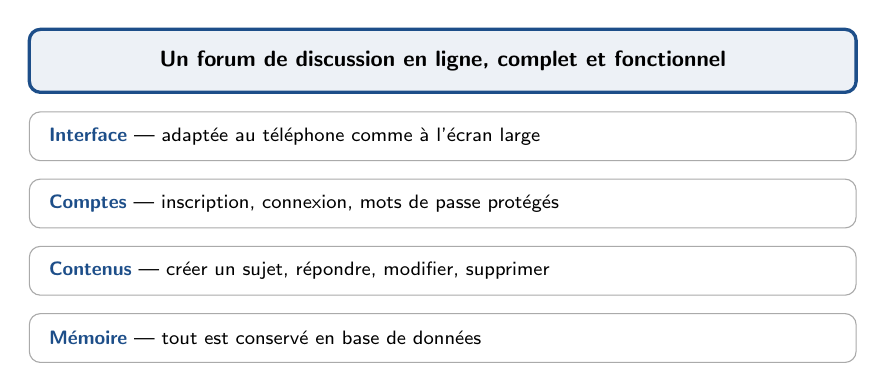
\begin{tikzpicture}[font=\scriptsize, node distance=0.22cm]
    \node[draw=accentBlue, very thick, rounded corners, fill=accentBlue!8,
          minimum width=10.5cm, minimum height=0.8cm, align=center] (a)
      {\footnotesize\textbf{Un forum de discussion en ligne, complet et fonctionnel}};
    \node[draw=cfptDarkGrey!50, rounded corners, fill=white,
          minimum width=10.5cm, minimum height=0.62cm, align=left,
          below=of a, text width=10cm] (b)
      {\textcolor{accentBlue}{\textbf{Interface}} --- adaptée au téléphone comme à l'écran large};
    \node[draw=cfptDarkGrey!50, rounded corners, fill=white,
          minimum width=10.5cm, minimum height=0.62cm, align=left,
          below=of b, text width=10cm] (c)
      {\textcolor{accentBlue}{\textbf{Comptes}} --- inscription, connexion, mots de passe protégés};
    \node[draw=cfptDarkGrey!50, rounded corners, fill=white,
          minimum width=10.5cm, minimum height=0.62cm, align=left,
          below=of c, text width=10cm] (d)
      {\textcolor{accentBlue}{\textbf{Contenus}} --- créer un sujet, répondre, modifier, supprimer};
    \node[draw=cfptDarkGrey!50, rounded corners, fill=white,
          minimum width=10.5cm, minimum height=0.62cm, align=left,
          below=of d, text width=10cm] (e)
      {\textcolor{accentBlue}{\textbf{Mémoire}} --- tout est conservé en base de données};
  \end{tikzpicture}
  \end{center}
  \vspace{-0.15cm}
  \begin{block}{Et vous saurez l'expliquer}
    \small La dernière séance est une soutenance : votre forum tourne en direct, et vous répondez aux questions sur votre propre code.
  \end{block}
\end{frame}

% --- 3. Le plan du cours ---
\begin{frame}{Le chemin que parcourt une information}
  \vspace{0.2cm}
  \begin{center}
  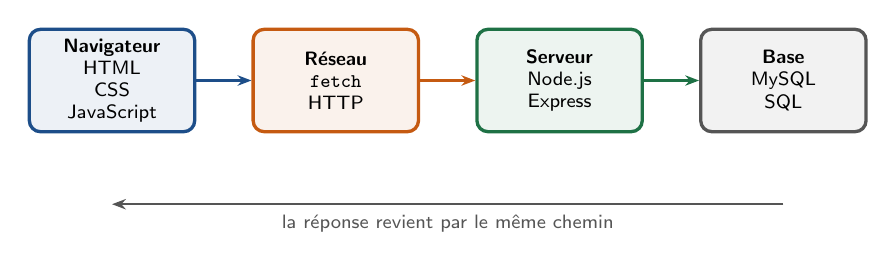
\begin{tikzpicture}[font=\scriptsize, node distance=0.7cm]
    \node[draw=accentBlue, very thick, rounded corners, fill=accentBlue!8,
          minimum width=2.1cm, minimum height=1.3cm, align=center] (nav)
      {\textbf{Navigateur}\\HTML\\CSS\\JavaScript};
    \node[draw=warningOrange, very thick, rounded corners, fill=warningOrange!8,
          minimum width=2.1cm, minimum height=1.3cm, align=center, right=of nav] (net)
      {\textbf{Réseau}\\\texttt{fetch}\\HTTP};
    \node[draw=successGreen, very thick, rounded corners, fill=successGreen!8,
          minimum width=2.1cm, minimum height=1.3cm, align=center, right=of net] (srv)
      {\textbf{Serveur}\\Node.js\\Express};
    \node[draw=cfptDarkGrey, very thick, rounded corners, fill=cfptGrey,
          minimum width=2.1cm, minimum height=1.3cm, align=center, right=of srv] (db)
      {\textbf{Base}\\MySQL\\SQL};
    \draw[-{Stealth[length=5pt]}, thick, accentBlue] (nav) -- (net);
    \draw[-{Stealth[length=5pt]}, thick, warningOrange] (net) -- (srv);
    \draw[-{Stealth[length=5pt]}, thick, successGreen] (srv) -- (db);
    \draw[-{Stealth[length=5pt]}, thick, cfptDarkGrey]
      ([yshift=-0.9cm]db.south)
      -- node[below, font=\scriptsize, text=cfptDarkGrey]
             {la réponse revient par le même chemin}
      ([yshift=-0.9cm]nav.south);
  \end{tikzpicture}
  \end{center}
  \vspace{0.35cm}
  \begin{block}{Ces quatre cases sont le plan du cours}
    On les apprend dans cet ordre, de gauche à droite. Chacune est un morceau du même projet, pas un exercice isolé.
  \end{block}
\end{frame}

% --- 4. Le parcours ---
\begin{frame}{Les 20 semaines}
  \vspace{0.35cm}
  \begin{center}
  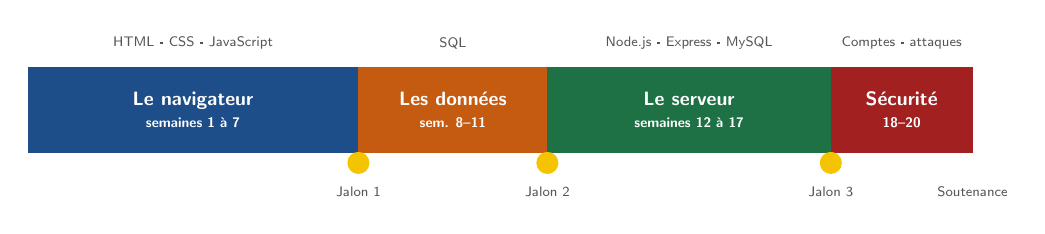
\begin{tikzpicture}[font=\scriptsize]
    % barres proportionnelles : 7 / 4 / 6 / 3 semaines sur 12 cm
    \fill[accentBlue]    (0,0)    rectangle (4.2,1.1);
    \fill[warningOrange] (4.2,0)  rectangle (6.6,1.1);
    \fill[successGreen]  (6.6,0)  rectangle (10.2,1.1);
    \fill[alertRed]      (10.2,0) rectangle (12,1.1);

    \node[text=white, font=\bfseries\scriptsize, align=center] at (2.1,0.55)
      {Le navigateur\\{\tiny semaines 1 à 7}};
    \node[text=white, font=\bfseries\scriptsize, align=center] at (5.4,0.55)
      {Les données\\{\tiny sem. 8--11}};
    \node[text=white, font=\bfseries\scriptsize, align=center] at (8.4,0.55)
      {Le serveur\\{\tiny semaines 12 à 17}};
    \node[text=white, font=\bfseries\scriptsize, align=center] at (11.1,0.55)
      {Sécurité\\{\tiny 18--20}};

    \foreach \x/\l in {4.2/Jalon 1, 6.6/Jalon 2, 10.2/Jalon 3} {
      \fill[cfptYellow] (\x,-0.12) circle (0.14);
      \node[font=\tiny, text=cfptDarkGrey, below] at (\x,-0.3) {\l};
    }
    \node[font=\tiny, text=cfptDarkGrey, below] at (12,-0.3) {Soutenance};

    \node[align=center, font=\tiny, text=cfptDarkGrey, above] at (2.1,1.2) {HTML · CSS · JavaScript};
    \node[align=center, font=\tiny, text=cfptDarkGrey, above] at (5.4,1.2) {SQL};
    \node[align=center, font=\tiny, text=cfptDarkGrey, above] at (8.4,1.2) {Node.js · Express · MySQL};
    \node[align=center, font=\tiny, text=cfptDarkGrey, above] at (11.1,1.2) {Comptes · attaques};
  \end{tikzpicture}
  \end{center}
  \vspace{0.7cm}
  \begin{columns}[T]
    \begin{column}{0.48\textwidth}
      \begin{block}{Chaque semaine}
        3 heures de théorie \quad + \quad 4 heures de pratique
      \end{block}
    \end{column}
    \begin{column}{0.48\textwidth}
      \begin{block}{Travail personnel}
        2 à 3 heures par semaine en dehors des cours
      \end{block}
    \end{column}
  \end{columns}
\end{frame}

% --- 5. Le fil rouge ---
\begin{frame}{Un seul projet, du premier au dernier jour}
  \vspace{0.2cm}
  \begin{center}
  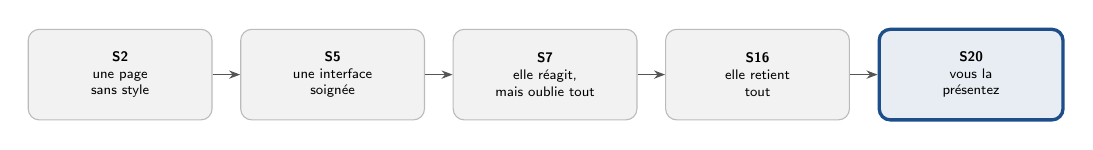
\begin{tikzpicture}[font=\tiny, node distance=0.35cm]
    \node[draw=cfptDarkGrey!40, rounded corners, fill=cfptGrey, text width=2.1cm,
          align=center, minimum height=1.15cm] (n1) {\textbf{S2}\\une page\\sans style};
    \node[draw=cfptDarkGrey!40, rounded corners, fill=cfptGrey, text width=2.1cm,
          align=center, minimum height=1.15cm, right=of n1] (n2) {\textbf{S5}\\une interface\\soignée};
    \node[draw=cfptDarkGrey!40, rounded corners, fill=cfptGrey, text width=2.1cm,
          align=center, minimum height=1.15cm, right=of n2] (n3) {\textbf{S7}\\elle réagit,\\mais oublie tout};
    \node[draw=cfptDarkGrey!40, rounded corners, fill=cfptGrey, text width=2.1cm,
          align=center, minimum height=1.15cm, right=of n3] (n4) {\textbf{S16}\\elle retient\\tout};
    \node[draw=accentBlue, very thick, rounded corners, fill=accentBlue!10, text width=2.1cm,
          align=center, minimum height=1.15cm, right=of n4] (n5) {\textbf{S20}\\vous la\\présentez};
    \foreach \a/\b in {n1/n2, n2/n3, n3/n4, n4/n5}
      \draw[-{Stealth[length=4pt]}, cfptDarkGrey] (\a) -- (\b);
  \end{tikzpicture}
  \end{center}
  \vspace{0.3cm}
  \centerline{\small Rien n'est jeté. Ce que vous écrivez en semaine 6 sert encore en semaine 20.}
  \vspace{0.4cm}
  \begin{exampleblock}{Si vous décrochez, vous pouvez remonter dans le train}
    \small À la fin des semaines 7, 11 et 17, je publie un forum conforme à ce qui était attendu. Si le vôtre est en difficulté, vous repartez du mien, sans pénalité pour la suite.
    \smallskip

    Prendre du retard est normal. Rester bloqué dehors ne l'est pas.
  \end{exampleblock}
\end{frame}

% --- 6. L'évaluation ---
\begin{frame}{Comment la note se construit}
  \vspace{0.2cm}
  \begin{center}
  \renewcommand{\arraystretch}{1.25}
  \begin{tabularx}{0.92\textwidth}{lXcc}
    \toprule
    \rowcolor{accentBlue}
    \color{white}\textbf{Épreuve} & \color{white}\textbf{Ce qui est évalué} &
    \color{white}\textbf{Sem.} & \color{white}\textbf{Poids} \\
    \midrule
    \rowcolor{cfptGrey}
    Jalon 1 & L'interface fonctionne dans le navigateur & 7 & 10\,\% \\
    Jalon 2 & Le modèle de données et les requêtes & 11 & 10\,\% \\
    \rowcolor{cfptGrey}
    Contrôle écrit & Individuel, sur machine, sans réseau & 12 & 25\,\% \\
    Jalon 3 & Le serveur est branché sur la base & 17 & 10\,\% \\
    \rowcolor{cfptGrey}
    Projet final & Le forum complet & 20 & 30\,\% \\
    Soutenance & Vous le présentez et l'expliquez & 20 & 15\,\% \\
    \bottomrule
  \end{tabularx}
  \end{center}
  \vspace{0.05cm}
  \begin{block}{Les jalons sont là pour vous, pas contre vous}
    \small Ils pèsent peu volontairement : leur rôle est de repérer tôt ce qui coince, pendant qu'il est encore temps d'y remédier.
  \end{block}
\end{frame}

% --- 7. La règle sur l'IA ---
\begin{frame}{L'intelligence artificielle générative est interdite}
  \vspace{0.2cm}
  \begin{alertblock}{La règle}
    Copilot, ChatGPT, Claude et les autres assistants qui écrivent du code sont interdits pour tous les travaux de ce cours.
  \end{alertblock}
  \vspace{0.35cm}
  \begin{columns}[T]
    \begin{column}{0.48\textwidth}
      \begin{block}{Pourquoi}
        \small On apprend à programmer en écrivant du code et en comprenant pourquoi il échoue. Un assistant qui donne la bonne réponse tout de suite supprime cette étape.
        \smallskip

        À hepia, les épreuves de programmation sont individuelles et sans assistance.
      \end{block}
    \end{column}
    \begin{column}{0.48\textwidth}
      \begin{block}{Ce qui reste autorisé}
        \small
        \begin{itemize}
          \item La documentation officielle (MDN)
          \item Les moteurs de recherche, les forums
          \item Vous entraider --- chacun écrit son code
        \end{itemize}
        \smallskip

        Je le vérifie par vos historiques Git et par des questions orales sur votre code.
      \end{block}
    \end{column}
  \end{columns}
\end{frame}

% --- 8. À quoi ça sert : le stage, puis hepia ---
\begin{frame}{À quoi ça va vous servir}
  \vspace{0.15cm}
  \begin{exampleblock}{D'abord au stage en entreprise --- 3\textsuperscript{e} trimestre}
    \small C'est l'échéance la plus proche, et celle où ce cours sert le plus directement. Vous y arriverez avec un projet complet à montrer, la capacité de lire du code existant et le vocabulaire pour suivre ce qui se dit autour de vous. C'est rare pour un stagiaire sans formation informatique.
  \end{exampleblock}
  \vspace{0.25cm}
  \begin{columns}[T]
    \begin{column}{0.46\textwidth}
      \begin{alertblock}{Ensuite à hepia --- soyons clairs}
        \small Le développement web n'y est pas enseigné en première année. Il arrive au semestre 4.
      \end{alertblock}
    \end{column}
    \begin{column}{0.5\textwidth}
      \begin{block}{Mais ce que vous emportez et pouvez transfèrer}
        \small L'habitude de découper un problème et d'écrire la suite d'instructions qui le résout.
        \smallskip

        C'est exactement ce qu'on vous demandera en \textbf{algorithmique et programmation}, votre matière la plus lourde en première année.
      \end{block}
    \end{column}
  \end{columns}
\end{frame}

% --- 9. Aujourd'hui ---
\begin{frame}{Concrètement, à partir de maintenant}
  \vspace{0.2cm}
  \begin{columns}[T]
    \begin{column}{0.48\textwidth}
      \begin{block}{Aujourd'hui}
        \begin{itemize}
          \item Comment fonctionne le web
          \item Installation de vos outils
          \item Création de votre dépôt Git
          \item Premier enregistrement du projet
        \end{itemize}
        \smallskip
        {\small Vous déposerez votre travail sur Git \textbf{à chaque séance} : c'est votre filet quand vous casserez quelque chose. Et vous casserez quelque chose.}
      \end{block}
    \end{column}
    \begin{column}{0.48\textwidth}
      \begin{block}{À votre disposition}
        \begin{itemize}
          \item Le plan de cours complet
          \item Un polycopié par semaine
          \item Les corrigés des exercices
        \end{itemize}
      \end{block}
      \vspace{0.2cm}
      \begin{exampleblock}{Une chose à retenir}
        \small Personne ne part avec de l'avance. Ce qui fera la différence en juin, c'est le nombre d'heures passées les mains dans le code --- pas le talent.
      \end{exampleblock}
    \end{column}
  \end{columns}
\end{frame}

% --- 10. Fin ---
{
\setbeamertemplate{footline}{}
\begin{frame}[plain]
  \begin{tikzpicture}[remember picture, overlay]
    \fill[accentBlue] (current page.north west) rectangle (current page.south east);
    \node[text=white, font=\Huge\bfseries] at ([yshift=0.6cm]current page.center) {Des questions ?};
    \fill[cfptYellow] ([yshift=-0.2cm]current page.center -| current page.west)
      rectangle ([yshift=-0.32cm]current page.center -| current page.east);
    \node[text=lightBlue, font=\large] at ([yshift=-1.3cm]current page.center)
      {On enchaîne : semaine 1 --- fondamentaux du web};
  \end{tikzpicture}
\end{frame}
}

\end{document}
